\chapter{Software Design}
\label{ch:software}

This chapter describes the software infrastructure that supports the \gls{vpu} design.
It covers the toolchain and build system, the Harvard memory model and its implications
for firmware writers, the firmware architecture of the UART-streaming applications, the
BT.601 grayscale benchmark that exercises the vector pipeline end-to-end, and the UART
communication protocol used for system-level testing.

% ===========================================================================
\section{Development Toolchain and Build System}
\label{sec:toolchain}

\subsection{Compiler and Assembler}

The firmware for this project is written in RISC-V assembly and assembled using the
\texttt{riscv64-unknown-elf-gcc} toolchain from the MSYS2 \texttt{mingw64} package set.
The assembler accepts the full \texttt{rv32im\_zicsr\_zve32x\_zvl128b} instruction set,
which is required to encode vector instructions such as \texttt{vsetvli} and
\texttt{vmulhu.vx} directly in assembly source files.

The compiler and assembler invocation uses the following flags:

\begin{itemize}
  \item \texttt{-march=rv32im\_zicsr\_zve32x\_zvl128b}: enables the base integer ISA
        (RV32I), the multiply/divide extension (M), the control and status register
        extension (Zicsr), the minimal vector extension for integer operations on 32-bit
        elements (Zve32x), and the 128-bit vector length body (Zvl128b).
  \item \texttt{-mabi=ilp32}: selects the 32-bit integer ABI, in which \texttt{int},
        \texttt{long}, and pointers are all 32 bits wide.
  \item \texttt{-mcmodel=medlow}: places all symbols in the low 2~GB address range
        (\texttt{0x00000000}–\texttt{0x7FFFFFFF}), allowing \texttt{lui}+\texttt{addi}
        two-instruction sequences for absolute address materialisation.
  \item \texttt{-Os}: optimises for code size. This prevents the compiler from emitting
        loop-unrolling or vectorisation code that is unnecessary in hand-written assembly.
  \item \texttt{-ffreestanding}: informs the compiler that there is no hosted standard
        library. This prevents the automatic insertion of calls to \texttt{\_\_main},
        \texttt{atexit}, or other runtime functions that are absent in the bare-metal
        environment.
  \item \texttt{-nostdlib -nostartfiles}: suppresses linking of the C standard library
        and the default startup object (\texttt{crt0.o}). The firmware provides its own
        \texttt{\_start} label that directly initialises the stack pointer and begins
        execution without any C runtime preamble.
  \item \texttt{-fno-builtin -fno-pic -fno-pie}: prevents automatic substitution of
        built-in library calls and disables position-independent code generation,
        both of which would introduce incorrect relocations in a single-load-address
        firmware image.
\end{itemize}

The toolchain is invoked from a GNU Makefile under MSYS2. A workaround is applied for
Windows temporary-directory handling: GCC on Windows uses the \texttt{TEMP}/\texttt{TMP}
environment variables rather than the MSYS2 \texttt{/tmp} mount, and the Makefile
explicitly creates a \texttt{../tmp} directory and exports its Windows-native path to
both variables before any compilation target is invoked.

\subsection{Build Flow}

The firmware build proceeds in four steps, summarised in
Figure~\ref{fig:build_flow}.

\begin{enumerate}
  \item \textbf{Assemble:} \texttt{gcc -c -o \$(SRC:.S=.o) \$(SRC)} — the assembly
        source is assembled into a relocatable object file (\texttt{.o}).
  \item \textbf{Link:} \texttt{gcc -Wl,-T link.ld -o \$(SRC:.S=.elf) \$(OBJ)} — the
        linker places the \texttt{.text} section at address \texttt{0x00000000} in IMEM
        and the \texttt{.bss} section at \texttt{0x00000000} in DMEM, as specified by
        \texttt{link.ld}.
  \item \textbf{Binary extraction:} \texttt{objcopy -O binary} converts the ELF image
        to a flat binary (\texttt{.bin}) whose first byte corresponds to the instruction
        at address zero.
  \item \textbf{Hex conversion:} The Python script \texttt{elf2hex\_lines.py} reads
        the binary and emits one 32-bit little-endian word per line in uppercase
        hexadecimal. This format is required by ModelSim's \texttt{\$readmemh} system
        function, which populates the IMEM array used by the \texttt{imem.sv} module.
\end{enumerate}

\begin{figure}[H]
  \centering
  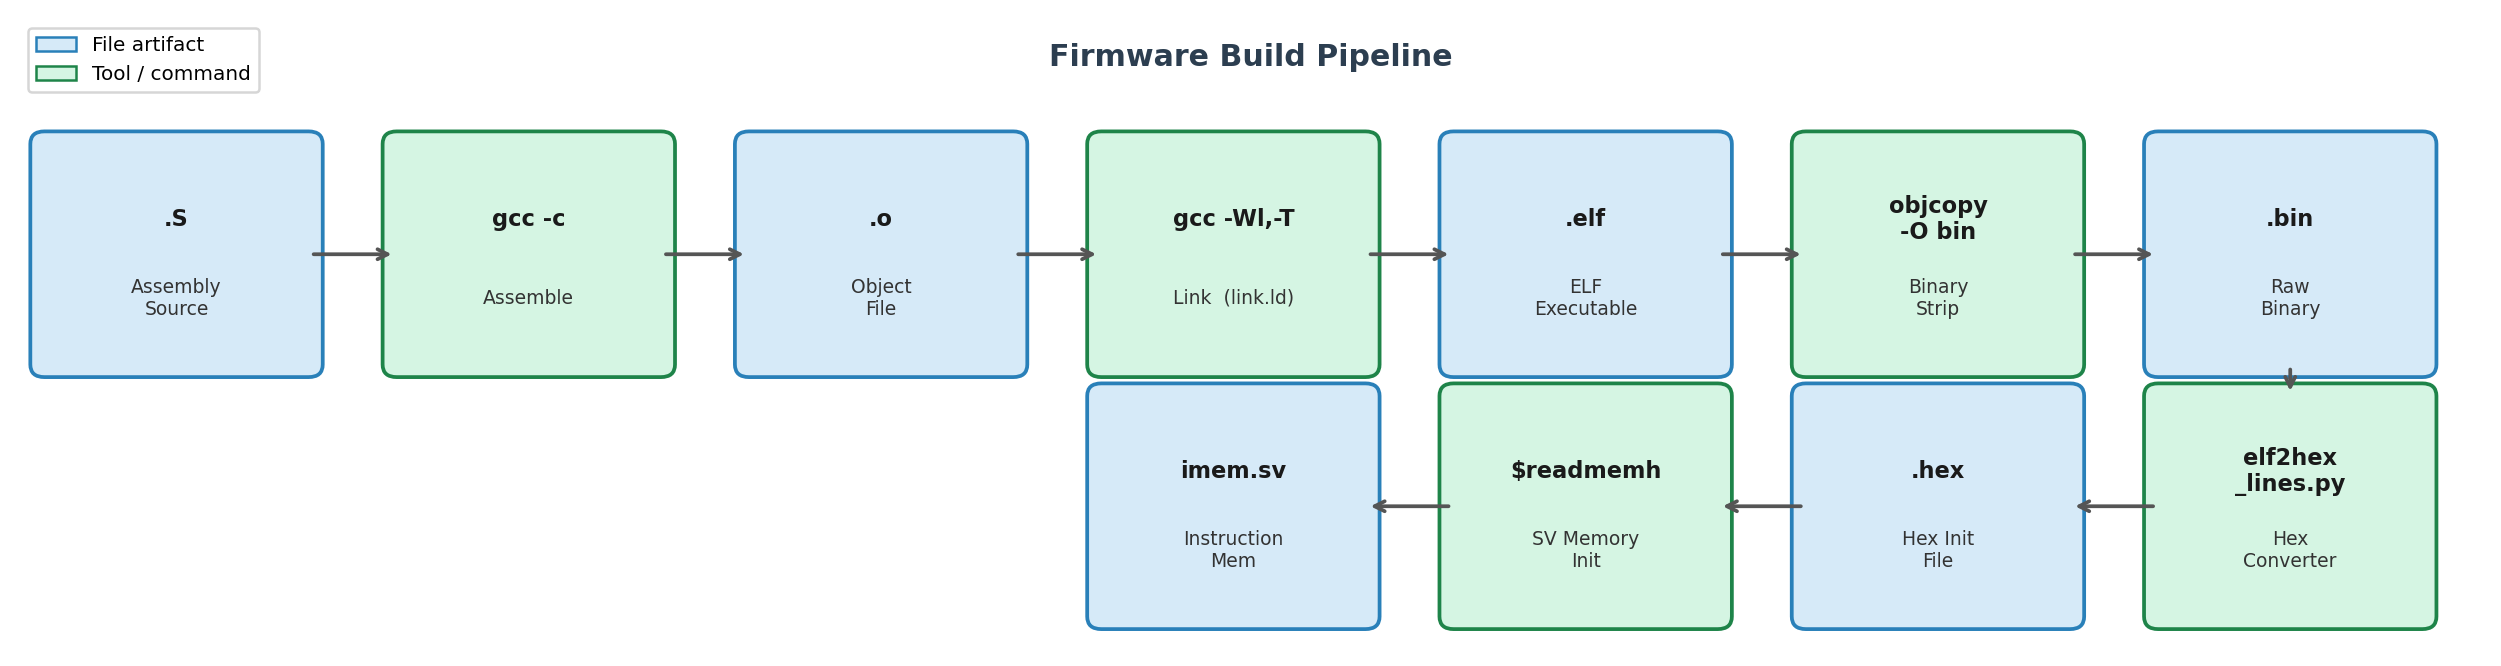
\includegraphics[width=\textwidth]{../image/build_flow.png}
  \caption{Firmware build flow diagram: .S source $\rightarrow$ .o (assemble) $\rightarrow$ .elf (link) $\rightarrow$ .bin (objcopy) $\rightarrow$ .hex (elf2hex\_lines.py) $\rightarrow$ \$readmemh in imem.sv}
  \label{fig:build_flow}
\end{figure}

\subsection{The \texttt{elf2hex\_lines.py} Converter}

ModelSim's \texttt{\$readmemh} directive expects one hexadecimal token per line, where
each token represents one memory word. The ELF binary produced by \texttt{objcopy}
contains raw bytes in little-endian order; a direct hexdump would produce one byte per
line rather than one 32-bit word per line. The \texttt{elf2hex\_lines.py} script
bridges this gap:

\begin{lstlisting}[language=Python, caption={elf2hex\_lines.py: binary-to-hex converter for \$readmemh}]
import struct, sys

def main():
    with open(sys.argv[1], "rb") as f:
        data = f.read()
    n = len(data) - (len(data) % 4)   # round down to word boundary
    for i in range(0, n, 4):
        (w,) = struct.unpack("<I", data[i : i + 4])   # LE 32-bit word
        print(f"{w:08X}")
\end{lstlisting}

The script reads groups of four bytes, interprets them as a 32-bit unsigned
little-endian integer using \texttt{struct.unpack("<I", ...)}, and prints each word
as an eight-character uppercase hexadecimal string. The output is redirected to
\texttt{imem.hex} (or a firmware-specific name such as \texttt{uart\_lena\_mini.hex})
and copied into the project root for simulation.

\subsection{Makefile Targets}

The Makefile in the \texttt{sw/} directory provides the following named targets, each
corresponding to a distinct firmware image:

\begin{table}[H]
  \centering
  \caption{Software build targets and their purposes}
  \label{tab:make_targets}
  \begin{tabular}{lll}
    \toprule
    \textbf{Target} & \textbf{Source file} & \textbf{Purpose} \\
    \midrule
    \texttt{all} (default) & \texttt{test\_alu.S} & Basic ALU smoke test \\
    \texttt{uart\_lena.hex} & \texttt{uart\_lena.S} & Full 128$\times$128 lena image, no echo \\
    \texttt{uart\_lena\_mini.hex} & \texttt{uart\_lena\_mini.S} & Single 16-pixel iteration for simulation \\
    \texttt{uart\_echo.hex} & \texttt{uart\_echo.S} & 16-pixel process + echo Y bytes + ACK \\
    \texttt{uart\_loopback.hex} & \texttt{uart\_loopback.S} & UART loopback test (no VPU) \\
    \texttt{disasm} & (any ELF) & Disassemble with \texttt{-Mnumeric -Mno-aliases} \\
    \bottomrule
  \end{tabular}
\end{table}

The \texttt{SRC} variable is overridable on the command line (\texttt{make SRC=uart\_echo.S})
so that any assembly source file can be built through the same four-step pipeline. A
separate \texttt{imem\_mifs} target invokes \texttt{make\_imem\_mifs.py} to generate the
four per-byte \texttt{.mif} initialisation files required by the Quartus
\texttt{altsyncram} ROM primitive used in the FPGA prototype.

% ===========================================================================
\section{Memory Model and Linker Script}
\label{sec:memory_model}

\subsection{Harvard Architecture Implications}

The system uses a strict Harvard memory architecture: the instruction memory (IMEM) and
data memory (DMEM) are separate address spaces, each with independent buses connecting
to the processor. The scalar core fetches instructions exclusively from IMEM; all
\texttt{lw}/\texttt{lh}/\texttt{lb} and \texttt{sw}/\texttt{sh}/\texttt{sb} instructions
address DMEM. The vector load/store unit (\gls{vlsu}) also addresses DMEM, and the
system provides a dual-port DMEM model (\texttt{dmem\_sync}) that exposes separate ports
for the scalar \gls{lsu} and the \gls{vlsu} to eliminate structural hazards.

The practical implication for firmware writers is that \texttt{.rodata} (read-only
constants such as string literals) must be placed in IMEM, but scalar \texttt{lw}
instructions cannot read from IMEM. Therefore, the firmware does not use any
\texttt{.rodata} constants accessed through pointers; all constants are materialised
as immediate literals in registers using \texttt{lui}/\texttt{addi} sequences or
single-cycle \texttt{li} pseudo-instructions.

\subsection{Linker Script}

The linker script \texttt{sw/link.ld} defines two memory regions:

\begin{lstlisting}[language=C, caption={Linker script (sw/link.ld) defining IMEM and DMEM regions}]
ENTRY(_start)
MEMORY {
  imem (rx) : ORIGIN = 0x00000000, LENGTH = 8K
  dmem (rw) : ORIGIN = 0x00000000, LENGTH = 2K
}

SECTIONS {
  .text : {
    *(.text.init)      /* _start must land at address 0 */
    *(.text .text.*)
  } > imem

  .rodata : { *(.rodata .rodata.*) } > imem

  .bss (NOLOAD) : {
    __bss_start = .;
    *(.bss .bss.*) *(COMMON)
    __bss_end = .;
  } > dmem
}
\end{lstlisting}

The IMEM region is marked \texttt{rx} (readable and executable) and occupies the
8~KB range \texttt{0x00000000}--\texttt{0x00001FFF}. The \texttt{.text.init} input
section is mapped first so that the reset vector at address zero jumps immediately to
\texttt{\_start}. The DMEM region is marked \texttt{rw} and occupies
\texttt{0x00000000}--\texttt{0x000007FF} (2~KB).

\subsection{Stack Size and Calling Convention}

The firmware stack pointer is initialised to \texttt{0x7F0} by the startup code and
grows downward toward lower addresses. A total of 16 bytes of stack space is sufficient
because all firmware functions are either leaf functions (they call nothing) or use the
\texttt{s1}/\texttt{ra} save pattern described in Section~\ref{sec:send_block} rather
than a conventional stack frame. No function allocates local variables on the stack,
and no register spilling occurs because the hand-written assembly is carefully written
to fit within the caller-saved temporary registers (\texttt{t0}--\texttt{t5}) without
exhausting them.

In the UART image-processing firmware, the callee-saved register \texttt{s0} permanently
holds the UART base address (\texttt{0xFF000000}) after the first \texttt{li} instruction
in \texttt{\_start}. Because \texttt{s0} is callee-saved under the RISC-V ABI, all
subroutines preserve it implicitly by never writing to it — a lightweight convention
that avoids the overhead of a full stack frame.

% ===========================================================================
\section{Firmware Architecture}
\label{sec:firmware_arch}

\subsection{Startup and Initialisation}

The firmware entry point is the \texttt{\_start} label, which the linker places at
IMEM address zero. There is no C runtime library, no exception vector table, and no
interrupt service routine. The only initialisation performed is loading the UART base
address into register \texttt{s0}:

\begin{lstlisting}[language=RISCV, caption={Firmware entry point: minimal initialisation}]
_start:
    li    s0, 0xFF000000    # UART base address (MMIO)
\end{lstlisting}

After this single instruction the firmware immediately begins executing the receive loop.
No stack pointer setup is needed because the firmware does not use the stack, and no BSS
zeroing is needed because the DMEM contents at the addresses used by the firmware are
overwritten before they are read.

\subsection{UART Register Map}

The UART peripheral is memory-mapped at base address \texttt{0xFF000000}. The firmware
accesses three registers:

\begin{table}[H]
  \centering
  \caption{UART MMIO register map}
  \label{tab:uart_mmio}
  \begin{tabular}{llll}
    \toprule
    \textbf{Offset} & \textbf{Name} & \textbf{Access} & \textbf{Description} \\
    \midrule
    \texttt{+0x04} & \texttt{STAT}  & RO & \texttt{[1]}=\texttt{RX\_VALID}, \texttt{[0]}=\texttt{TX\_BUSY} \\
    \texttt{+0x08} & \texttt{TXDAT} & WO & Write byte to transmit FIFO \\
    \texttt{+0x0C} & \texttt{RXDAT} & RO & Read and dequeue one received byte \\
    \bottomrule
  \end{tabular}
\end{table}

\texttt{RX\_VALID} (bit~1 of \texttt{STAT}) is set when at least one byte is available
in the receive FIFO. The firmware polls this bit in a busy-wait loop before reading
\texttt{RXDAT}; reading \texttt{RXDAT} automatically dequeues one byte.
\texttt{TX\_BUSY} (bit~0 of \texttt{STAT}) is set while the transmitter is serialising
a byte; the firmware polls it before writing the next byte to \texttt{TXDAT}.

\subsection{The \texttt{recv\_block} Subroutine}

\texttt{recv\_block} receives a burst of bytes from the UART and stores them
sequentially in DMEM, starting at byte address \texttt{a0} for a count of \texttt{a1}
bytes. The algorithm is:

\begin{lstlisting}[language=RISCV, caption={recv\_block: receive a1 bytes from UART into DMEM at address a0}]
recv_block:
    add   t0, a0, a1         # t0 = end address (a0 + count)
recv_loop:
    bge   a0, t0, recv_done  # loop until a0 reaches end
rx_wait:
    lw    t1, 4(s0)          # read STAT register
    andi  t1, t1, 2          # isolate RX_VALID bit
    beqz  t1, rx_wait        # spin if no byte available
    lw    t1, 12(s0)         # read RXDAT (dequeues byte)
    sb    t1, 0(a0)          # store byte to DMEM
    addi  a0, a0, 1          # advance DMEM pointer
    j     recv_loop
recv_done:
    ret
\end{lstlisting}

The \texttt{lw} instruction reads four bytes from the MMIO address, but only the
low byte of \texttt{RXDAT} contains the received character; the \texttt{sb} instruction
naturally discards the upper three bytes. The \texttt{bge} branch at the top of the
loop checks a signed comparison, which is correct because all DMEM addresses and counts
used by the firmware are non-negative and fit within 31 bits.

\subsection{The \texttt{uart\_tx\_byte} Subroutine}

\texttt{uart\_tx\_byte} transmits the single byte held in \texttt{a0[7:0]} via the
UART TX channel. It polls \texttt{TX\_BUSY} before writing:

\begin{lstlisting}[language=RISCV, caption={uart\_tx\_byte: transmit one byte (a0[7:0]) via UART}]
uart_tx_byte:
tx_wait:
    lw    t0, 4(s0)          # read STAT
    andi  t0, t0, 1          # isolate TX_BUSY bit
    bnez  t0, tx_wait        # spin if transmitter busy
    sw    a0, 8(s0)          # write byte to TXDAT
    ret
\end{lstlisting}

The \texttt{sw} writes a full 32-bit word to \texttt{TXDAT}; the UART peripheral uses
only the low 8 bits. After the write, the UART controller asserts \texttt{TX\_BUSY}
on the next clock edge and begins serialising the byte.

\subsection{The \texttt{send\_block} Subroutine}
\label{sec:send_block}

\texttt{send\_block} transmits a sequence of \texttt{a1} bytes starting at DMEM
byte address \texttt{a0}. Because it calls \texttt{uart\_tx\_byte} internally, a
standard \texttt{call}/\texttt{ret} pattern would overwrite the return address register
(\texttt{ra}) when the nested \texttt{call uart\_tx\_byte} is executed. Rather than
allocating a stack frame, the firmware saves \texttt{ra} into the callee-saved register
\texttt{s1} at the start of the subroutine and restores it before returning:

\begin{lstlisting}[language=RISCV, caption={send\_block: send a1 bytes from DMEM address a0 via UART}]
send_block:
    mv    s1, ra             # save caller's return address in s1
    mv    t2, a0             # t2 = current byte pointer
    add   t3, a0, a1         # t3 = end pointer
send_loop_b:
    bge   t2, t3, send_done_b
    lbu   a0, 0(t2)          # load byte (zero-extended) into a0
    call  uart_tx_byte       # transmits a0[7:0]; overwrites ra
    addi  t2, t2, 1
    j     send_loop_b
send_done_b:
    mv    ra, s1             # restore caller's return address
    ret
\end{lstlisting}

The \texttt{lbu} (load byte unsigned) instruction is used rather than \texttt{lb} to
ensure that the byte value is zero-extended into \texttt{a0}, which prevents the
transmission of a sign-extended 32-bit value when the byte has its MSB set. This is
important for image data where pixel values range from 0 to 255; without zero-extension,
a pixel value of 200 (binary \texttt{11001000}) would appear to the UART as
\texttt{0xFFFFFFC8}, and only the low byte would be transmitted correctly — but relying
on that truncation would be fragile.

The \texttt{s1} save pattern is safe because the call chain in this firmware does not
use \texttt{s1} for any other purpose: \texttt{\_start} does not call \texttt{send\_block}
and \texttt{uart\_tx\_byte} simultaneously, and \texttt{uart\_tx\_byte} is itself a leaf
function that does not modify \texttt{s1}.

% ===========================================================================
\section{Application: BT.601 Grayscale Conversion}
\label{sec:bt601}

\subsection{Background: ITU-R BT.601 Luma Formula}

The ITU-R BT.601 standard defines the conversion from analogue component video to
digital luminance and chrominance. The luma channel $Y$ for a pixel with red, green,
and blue components $(R, G, B) \in [0, 255]$ is:

\begin{equation}
  Y = \bigl\lfloor R \times 0.299 \bigr\rfloor +
      \bigl\lfloor G \times 0.587 \bigr\rfloor +
      \bigl\lfloor B \times 0.114 \bigr\rfloor
  \label{eq:bt601_float}
\end{equation}

For efficient fixed-point implementation, the fractional weights are approximated by
integer fractions with a power-of-two denominator. With 256 as the denominator, the
integer coefficients become $77$, $150$, and $29$, which satisfy:

\begin{equation}
  Y = \Bigl\lfloor \frac{R \times 77}{256} \Bigr\rfloor +
      \Bigl\lfloor \frac{G \times 150}{256} \Bigr\rfloor +
      \Bigl\lfloor \frac{B \times 29}{256} \Bigr\rfloor
  \label{eq:bt601_fixed}
\end{equation}

The coefficients satisfy $77 + 150 + 29 = 256$, so the maximum value of $Y$ for a
white pixel ($R=G=B=255$) is $255 \times 256 / 256 = 255$. In practice the hardware
sum is $\lfloor 255 \times 77/256 \rfloor + \lfloor 255 \times 150/256 \rfloor +
\lfloor 255 \times 29/256 \rfloor = 76 + 149 + 28 = 253$, which is the expected
integer result due to the three floor operations.

\subsection{Mapping to \texttt{vmulhu.vx}}

The key insight that makes this algorithm efficient on the VPU is the mapping of the
division-by-256 to the upper byte of an 8-bit unsigned multiply. For two 8-bit unsigned
operands $a, b \in [0, 255]$, the 16-bit product $p = a \times b$ satisfies:

\begin{equation}
  \Bigl\lfloor \frac{a \times b}{256} \Bigr\rfloor = p[15:8]
\end{equation}

The RVV instruction \texttt{vmulhu.vx} with \texttt{SEW=8} computes, for each element
$i$, the upper byte of the 16-bit unsigned product of the vector element and a scalar
register. This is exactly the operation needed: \texttt{vmulhu.vx v4, v1, t3}
computes \texttt{v4[i] = (v1[i] * t3)[15:8]} for each $i$, which is
\texttt{v4[i] = floor(R[i] * 77 / 256)}. No explicit right-shift or division instruction
is required; the truncation is implicit in the high-half extraction.

\subsection{Full Instruction Sequence}

The complete BT.601 kernel for 16 pixels processes a single VLMAX-sized group in the
following instruction sequence:

\begin{lstlisting}[language=RISCV, caption={BT.601 grayscale VPU kernel: 16 pixels per iteration at SEW=8 LMUL=1}]
    # Scalar setup: load coefficients and base addresses
    li    t3, 77                     # R weight
    li    t4, 150                    # G weight
    li    t5, 29                     # B weight
    li    t1, 16
    vsetvli t1, t1, e8, m1, ta, ma  # vl=16, SEW=8, LMUL=1

    # Vector load: read 16-element groups from DMEM
    vle8.v    v1, (a0)               # load R[0..15]
    vle8.v    v2, (a1)               # load G[0..15]
    vle8.v    v3, (a2)               # load B[0..15]

    # Vector multiply: vmulhu.vx extracts upper byte of 8x8 product
    vmulhu.vx v4, v1, t3             # v4[i] = floor(R[i]*77/256)
    vmulhu.vx v5, v2, t4             # v5[i] = floor(G[i]*150/256)
    vmulhu.vx v6, v3, t5             # v6[i] = floor(B[i]*29/256)

    # Vector add: accumulate Y = Yr + Yg + Yb
    vadd.vv   v7, v4, v5             # v7[i] = Yr[i] + Yg[i]
    vadd.vv   v7, v7, v6             # v7[i] += Yb[i]  => Y[i]

    # Vector store: write 16 luminance bytes to DMEM
    vse8.v    v7, (a3)               # store Y[0..15] to 0xC000
\end{lstlisting}

\texttt{vsetvli} configures the VPU with \texttt{e8} (element width 8 bits),
\texttt{m1} (LMUL=1, one register group), \texttt{ta} (tail-agnostic), and \texttt{ma}
(mask-agnostic). With VLEN=128 bits and SEW=8, VLMAX=128/8=16, so \texttt{vl} is set
to 16 and \texttt{t1} is written with the confirmed active vector length.

The full 128$\times$128 image requires $128 \times 128 / 16 = 1024$ iterations of
this kernel. Each iteration issues exactly nine vector instructions (one
\texttt{vsetvli}, three \texttt{vle8.v}, three \texttt{vmulhu.vx}, two \texttt{vadd.vv},
one \texttt{vse8.v}) plus overhead loads of base addresses. The benchmark result of
34828 cycles for 16384 pixels yields approximately 34 cycles per 16-element group, or
2.1 cycles per pixel.

\subsection{Throughput Analysis}

Table~\ref{tab:vpu_throughput} shows the per-instruction cycle counts observed in
simulation. The VPU processes one SEW-wide element per clock cycle in its execution
lane; for SEW=8 and vl=16, each arithmetic instruction therefore completes in exactly
16 execution cycles plus a small fixed decode and writeback overhead.

\begin{table}[H]
  \centering
  \caption{VPU instruction cycle counts for SEW=8, vl=16}
  \label{tab:vpu_throughput}
  \begin{tabular}{lcc}
    \toprule
    \textbf{Instruction} & \textbf{Execution cycles} & \textbf{Elements/cycle} \\
    \midrule
    \texttt{vsetvli}   & 1  & N/A \\
    \texttt{vle8.v}    & 16 & 1 \\
    \texttt{vmulhu.vx} & 16 & 1 \\
    \texttt{vadd.vv}   & 16 & 1 \\
    \texttt{vse8.v}    & 16 & 1 \\
    \bottomrule
  \end{tabular}
\end{table}

A na\"ive scalar implementation of the same kernel would require approximately 80 cycles
per pixel group: one \texttt{mul} (3 cycles), one \texttt{srl} (1 cycle), and one
\texttt{sb} (2 cycles) per channel, repeated three times per pixel, for 16 pixels.
The VPU processes the same 16 pixels in roughly 16 cycles for each of the five
arithmetic/memory stages, yielding a throughput advantage of approximately 16$\times$
for the arithmetic portion.

\subsection{Accuracy Analysis}

The hardware implementation is bit-exact with the formula in Equation~\ref{eq:bt601_fixed}.
The \texttt{vmulhu.vx} instruction with SEW=8 computes the integer floor of the product
divided by 256 by construction (the upper byte of a 16-bit product is exactly the floor
of the 16-bit value divided by 256). There is no rounding error, no saturation, and no
intermediate truncation. The system-level testbench \texttt{tb\_uart\_echo.sv} verifies
this by comparing all 16 computed Y values against a reference implementation in
SystemVerilog that uses the same formula, and 16/16 pixel comparisons pass with zero
error for all test vectors.

% ===========================================================================
\section{UART Communication Protocol}
\label{sec:uart_protocol}

\subsection{Physical Layer Parameters}

The UART peripheral operates at a baud rate of 115200 baud with 8 data bits, no parity,
and one stop bit (8N1). In the simulation environment the system clock is set to
14.745600~MHz, which gives an exact 128:1 ratio between the clock frequency and the
baud rate (the UART divider register is set to 7, yielding a $\times$8 oversampling
factor of 8 clocks per bit). This exact ratio eliminates fractional baud-rate error
and ensures that simulation results are directly representative of hardware behaviour.

\subsection{Image Streaming Protocol}

The host-to-device protocol for the BT.601 application is:

\begin{enumerate}
  \item Host transmits 16 (or 16384) R-channel bytes sequentially, most-significant
        first within each row. The firmware stores these directly to DMEM starting at
        address \texttt{0x0000}.
  \item Host transmits 16 (or 16384) G-channel bytes. The firmware stores these to DMEM
        at address \texttt{0x4000}.
  \item Host transmits 16 (or 16384) B-channel bytes. The firmware stores these to DMEM
        at address \texttt{0x8000}.
  \item The firmware invokes the VPU kernel and stores the resulting Y bytes to DMEM at
        \texttt{0xC000}.
\end{enumerate}

Transmitting the three colour planes in sequential order (rather than interleaved as
RGB triples) simplifies the firmware loop structure: each call to \texttt{recv\_block}
handles a single contiguous DMEM segment, and the VPU vector loads of the three channels
are independent, allowing the scalar core to issue them without stall cycles.

\subsection{Echo and Acknowledgement}

The \texttt{uart\_echo.S} firmware extends the basic protocol with a return path. After
completing the VPU computation, the firmware transmits all 16 computed Y bytes back to
the host using \texttt{send\_block}, followed by a single acknowledgement byte
\texttt{0xAA}. This allows the testbench or a host software application to verify
the computation result over a fully serial path without needing direct DMEM access.

The choice of \texttt{0xAA} as the ACK value is deliberate: it alternates between 0 and
1 in binary (\texttt{10101010}), which provides a good oscilloscope pattern for baud-rate
verification and is easy to distinguish from any valid image pixel value (which ranges
from 0 to 253 for BT.601 luma).

\subsection{Timing Budget}

At 115200 baud with 8N1 framing, each byte occupies $10/115200 \approx 86.8~\mu$s on
the wire. For the 16-pixel echo protocol, the total byte count is:

\begin{itemize}
  \item Receive: 16 (R) + 16 (G) + 16 (B) = 48 bytes
  \item Transmit: 16 (Y) + 1 (ACK) = 17 bytes
  \item Total: 65 bytes $\times$ 86.8~$\mu$s $\approx$ 5.6~ms
\end{itemize}

In the simulation, each bit takes 8 clock cycles at 14.745600~MHz (0.54~$\mu$s per bit),
so 65 bytes of 10-bit-framed UART data occupy $65 \times 10 \times 8 = 5200$ clock
cycles, plus several hundred cycles for VPU processing, giving a total well within the
50000-cycle simulation timeout.

% ===========================================================================
\section{Summary}
\label{sec:software_summary}

This chapter described the firmware infrastructure built on top of the RISC-V VPU.
The toolchain build flow produces IMEM-ready hex images from assembly source files
through a four-step pipeline: assemble, link, binary-strip, and hex-convert. The linker
script enforces the Harvard separation between IMEM (\texttt{.text} and \texttt{.rodata}
at address 0) and DMEM (\texttt{.bss} at address 0), and the absence of a C runtime
library is accommodated by providing a bare-metal \texttt{\_start} entry point with
minimal initialisation.

The BT.601 grayscale kernel demonstrates that the RVV \texttt{vmulhu.vx} instruction
maps directly to the fixed-point luma formula, processing 16 pixels per vector
instruction with zero quantisation error. The UART communication protocol provides an
end-to-end data path from host to VPU and back, enabling pixel-accurate regression
testing of the full hardware stack.
